\section{Directed Team Graph (DiTG)}

In order to measure human workload within the context of our model \cite{gledhill2013modelinguas} we
have defined the following set of core components which allows us to correlate
the activity within our model to human workload. 

\subsection{Conceptual Model}
As described in the previous section, we modeled a WiSAR team as a collection of directed role graphs
(DiRGs).  This collection, illustrated in Figure~\ref{fig:ditg}, is essentially a graph, and we can augment the edges of this graph with information that allows us to track workload.  We call this graph a {\em Directed Team Graph} (DiTG), and note that this graph formalizes this collection by defining the communication mediums which
unite the said Actors.  Using multiple resource theory \cite{wickens2002multiple}
as a guide we can explicitly define the channels over which this communication occurs (see Figure~\ref{fig:ditg_detail}).  The Actor state transitions then use these
channels to broadcast and receive inter-actor communication.  

We hope to gain
insight into decreasing the system workload, and possibly combining roles, by
establishing metrics associated with the system model and model simulation. 
These metrics can then be used to determine if changes to the model represent a
decrease in operator workload.

\begin{figure}
\center
\setlength{\abovecaptionskip}{1mm}
\setlength{\belowcaptionskip}{1mm}
\setlength{\textfloatsep}{1mm}
\setlength{\floatsep}{1mm}
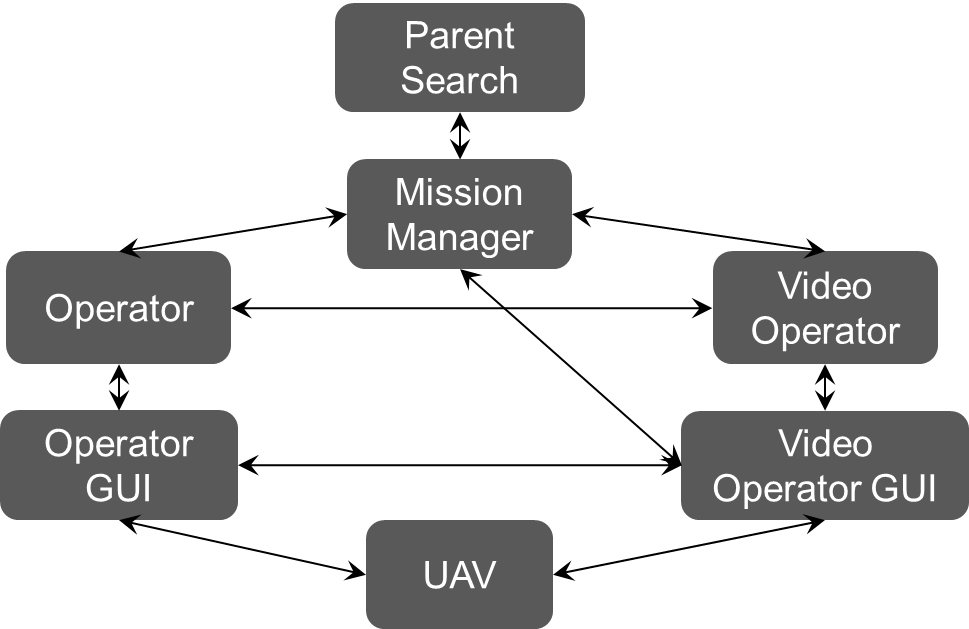
\includegraphics[height=2in]{ditg.png}
\caption{High Level DiTG}
\label{fig:ditg}
\end{figure}

\begin{figure}
\center
\setlength{\abovecaptionskip}{1mm}
\setlength{\belowcaptionskip}{1mm}
\setlength{\textfloatsep}{1mm}
\setlength{\floatsep}{1mm}
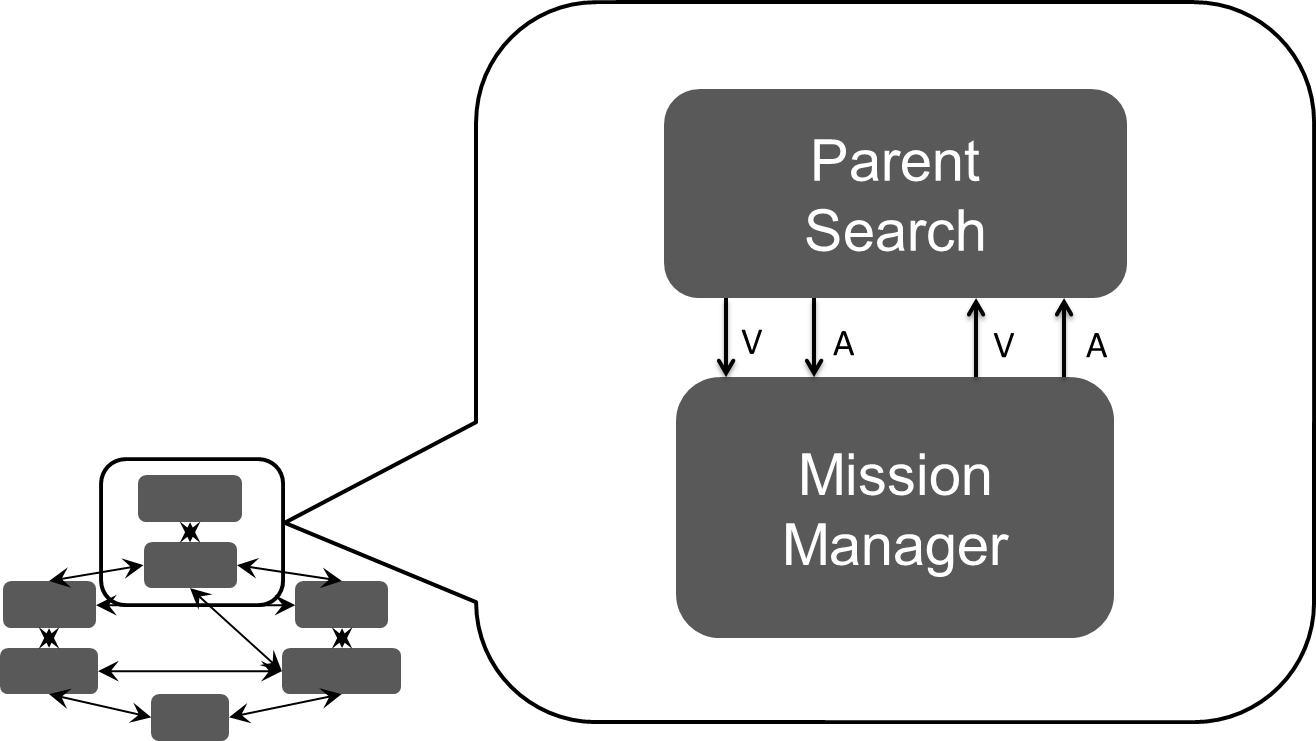
\includegraphics[height=1.9in]{ditg_detailed.png}
\caption{Detail view of DiTG: V is a Visual channel and A is an Audio channel}
\label{fig:ditg_detail}
\end{figure}

Formally, the framework is the following mathematical structures:
 \begin{equation}
 	DiTG = (A, \Phi, \forall a_i \in A~ \exists \Phi_i \subset \Phi)
 \end{equation}

% \begin{equation}
% 	Actor = (S, s_0, s_{current}, \Omega_A, \Sigma_A \subset \Phi, \Lambda_A
% 	\subset \Phi)
 %\label{eq:actor}
 %\end{equation}
%
% \begin{equation}
%	State = (T_{enabled}, T_{disabled}) : T_{enabled} \cap T_{disabled} = \emptyset
% \label{eq:state}
%\end{equation}
%
%\begin{equation}
%\begin{split}
%	Transition = (\Omega_{input} \subset \Omega_A, \Sigma_{input} \subset \Sigma_A,\\
%	\Omega_{value}^{input}, \Sigma_{value}^{input} \\
%	\Omega_{output} \subset \Omega_A, \Lambda_{output} \subset \Lambda_A, \\
%	\Omega_{value}^{output}, \Lambda_{value}^{output}, duration)
% \label{eq:transition}
% \end{split}
%\end{equation}

\begin{equation}
\begin{split}
Channel (\phi) = (type \in (visual, audio), \\
value \in (null, *), 
 a_i^{source}, a_j^{target}) : i \neq j
 \label{eq:channel}
 \end{split}
\end{equation}

\begin{equation}
Declarative Memory(\omega) = value \in (null, *)
\end{equation}


\noindent where $A$ is a set of actors, $S$ a set of
states, $T$ a set of transitions, $\Phi$ a set of channels, $\Omega$ a set of
declarative memory, $\Sigma$ a set of input channels, and $\Lambda$ a set of
output channels.

\subsection{Framework Components}
\subsubsection{Actors}
Actors represent the agents within the system, while an Actor may be any type of
agent for the context of workload we assume that an Actor is human.  An Actor is
made up of an initial state, a current state, the set of all possible states,
declarative memory, input channels and output channels.  They are represented
within the model as finite state machines expressed by DiRGs.

\subsubsection{States}
States contain two sets of Actor transitions, enabled and disabled, which
represent all possible transitions the Actor can follow while in that state. 
While states typically represent the performance of a set of tasks they can also
represent such things as emotion, fatigue, and neglect which is expressed in the
transitions.  In this way an Actor's current state represents its current
decision making paradigm.

\subsubsection{Transitions}
A transition is composed of a set of required declarative memory and channel
values, a set of declarative memory and channel output values, an end state, and
a duration.  A transition is considered enabled when all of its input
requirements are met.  The duration represents the relative difficulty of the
task(s) associated with the transition.  We rationalize this by assuming that
all tasks are performed at a constant rate, thus more difficult tasks take
longer.  It should be noted that our initial models also included transition
priority and probability, however, we are ignoring these attributes to simplify
our first order workload metrics.

\subsubsection{Declarative Memory }
This memory represents internal facts stored by an Actor and used in decision
making.  This memory takes the form of internal variables within an Actor. 
Transitions can look for specific values on these variables to determine if they are enabled.

\subsubsection{Channels} 
Channels represent physical communication mediums that exist between Actors. 
Each channel has a type (audio or visual), a buffer, a source, and a target. 
The channel type is associated with the modality dimension of multiple resource
theory while the source and target represent the stages
dimension \cite{wickens2002multiple}.  The source being the response and the
target being perception/cognition.  We assume that all channels have a constant
bandwidth, the longer a channel is in use the more data being sent across the channel.  

\subsubsection{How it works}
We represent a system as a DiTG, a collection of
Actors connected to one another by a set of channels.  Whenever the state of the
system changes an Actor will petition, from its current state, a list of enabled
transitions thus defining what decisions can be made.  The Actor may then
activate one of these transitions.  Transitions have two main states, active and
fired.  When chosen a transition is made active, after the specified duration
the transition fires.  When a transition becomes active it creates temporary
output values for declarative memory and channels.  These temporary values are
then applied to the actual declarative memory and channel values once the transition fires.

\subsection{Actor vs Tasks}
This architecture focuses on the Actor itself and less on the tasks performed by
the Actor.  The difference being that Actor states can account for conditions on
the Actor which affect performance and increase workload which cannot be seen
simply by taking a set of tasks and examining their combined resource
requirements.  For our model we never explicitly define a single task.  Instead
we define Actors, States, and Transitions.  Each transition defines its own
perceptual, cognitive, response, and declarative resources \cite{salvucci2008threaded} which are
not restricted to performing a single task.  In this way an Actor's state
determines what task(s) are being performed, achieving multi-tasking without
explicitly defining tasks.  The value of this distinction goes much higher. 
States can also represent different physical, emotional, or other conditions
through adding/removing states and through changes to state transitions. One
example is to increase transition durations to represent fatigue.
Comparing workload profiles for multiple scenarios using multiple
similar models may give insight into what scenarios create higher user workload.

\subsection{Model Creation}
To simplify the modeling process and ensure rigorous model creation we
developed a transition language, similar to a Kripke structure, which allows
models to be expressed as a list of Actor transitions.  A parser then
automatically generates the classes required to run the model simulation.
The transition language uses the following structure.
\begin{equation}
\begin{split}
(s_{current}, [\phi_{input} = value,\ldots], [\omega_{input} = value,\ldots],\\
duration) \times \\
(s_{next}, [\phi_{output} =
value,\ldots], [\omega_{output} = value,\ldots])
\end{split}
\end{equation}
\noindent The language is compiled to a Java program suitable to run standalone
as a simulation or analyzed by the JPF model checker to create
workload profiles.
